\documentclass{boi2014-de}

\usepackage{enumitem}
\usepackage{todonotes}
\usepackage{wrapfig}
\usepackage{mathtools}
\usepackage{tikz}

\renewcommand{\DayNum}{1}
\renewcommand{\TaskCode}{coprobber}
\renewcommand{\TaskName}{Räuber und Gendarm}
\renewcommand{\TaskVersion}{1.4}

\renewcommand{\labelitemii}{$\circ$}
\newcommand{\constant}[1]{{\tt #1}}

\begin{document}
    \begin{wrapfigure}{r}{6cm}
		\includegraphics[width=6cm]{\TaskCode.jpeg}
	\end{wrapfigure}

    In Bytemore City sind die Räuber auf dem Vormarsch!  Und nach jedem Raub
    ist es die Aufgabe eines einsamen Gendarmen, den Räuber durch die engen Straßen
    der Stadt zu verfolgen, die die Kreuzungen miteinander verbinden.
    Dummerweise entkommen die Räuber häufig, da sie die Stadt viel besser kennen als die Gendarmen.

    Das Bytemore City Police Department (BCPD) will nun Computer einsetzen,
    um das Verbrechen besser zu bekämpfen. Das BCPD hat dazu bereits einen präzisen
    Stadtplan von Bytemore City angefertigt. Nun wird noch Software benötigt,
    die Strategien zur Verfolgung von Räubern ermitteln soll.

    In der Software wird die Verfolgung eines Räubers durch einen Gendarmen so modelliert:
    \begin{enumerate}
        \item 
        Der Gendarm wählt eine Kreuzung, von der aus er beginnt.
        \item 
            Der Räuber kennt nun die Position des Gendarmen und wählt eine Kreuzung für den Raub.
            Von da an kennen Räuber und Gendarm gegenseitig ihre Position.
        \item 
            Nun ist der Gendarm am Zug.  Er kann sich über eine Straße zu einer benachbarten Kreuzung bewegen 
            oder warten (und sich nicht bewegen).
        \item 
            Nun ist der Räuber am Zug.  Er bewegt sich in jedem Zug über eine Straße zu einer benachbarten Kreuzung.
            Beachte: Räuber können einfach nicht warten, das Weglaufen gehört zum Berufsethos.
        \item 
        Nun ziehen Gendarm und Räuber abwechselnd (der Gendarm beginnt),
        bis eines der folgenden Dinge passiert:
        
        \begin{enumerate}
            \item 
                Ein Zustand (gegeben durch die Positionen von Räuber und Gendarm und die
                Angabe, wer als nächster am Zug ist) wiederholt sich.
                Der Räuber kann also dem Gendarmen beliebig lange aus dem Weg gehen und entkommt so.
            \item 
                Nach einem Zug befinden sich Räuber und Gendarm auf derselben Kreuzung.
                In diesem Fall ist der Räuber gefangen.
        \end{enumerate}
    \end{enumerate}

    \Task
    Schreibe ein Programm, das bei gegebenem Stadtplan bestimmt,
    ob der Räuber gefangen werden kann, und, falls ja, die dazu nötigen Züge des Gendarmen angibt.

    Dein Programm soll annehmen, dass der Räuber optimale Züge macht.

    \Implementation
    Du musst zwei Funktionen implementieren:
    \begin{itemize}
        \item \method{start(N, A)} mit den folgenden Parametern:
            \begin{itemize}
                \item $N$ -- die Anzahl der Kreuzungen (nummeriert von $0$ bis $N-1$);
                \item $A$ -- ein zweidimensionales Array, das die Straßen beschreibt:
                    für $0 \le i, j \le N-1$,
                    $$
                        A[i, j] \text{ ist }
                        \begin{dcases*}
                            \texttt{false} & falls $i$ und $j$ nicht durch eine Straße verbunden sind.
                                \\
                            \texttt{true} & falls $i$ und $j$ durch eine Straße verbunden sind.
                        \end{dcases*}
                    $$
                    Alle Straßen sind in beiden Richtungen begehbar (also $A[i, j] = A[j, i]$ für alle $i, j$),
                    und es gibt keine ``Schleifen'' (also: $A[i, i]$ ist \texttt{false} für alle $i$).
                    Außerdem gilt: Für jede Kreuzung gibt es einen Weg zu jeder anderen Kruezung über die Straßen.
            \end{itemize}
        
        Falls der Räuber in dem durch den Stadtplan gegebenen Straßennetz gefangen werden kann,
        soll die Funktion \method{start} die Nummer der Kreuzung zurückgeben, die der Gendarm als seinen Startpunkt wählen sollte. Sonst soll sie $-1$ zurückgeben.

        \item \method{nextMove(R)} 
            nimmt als Parameter die Nummer $R$ der Kreuzung, auf der sich der Räuber gerade befindet.
            Sie liefert die Nummer der Kreuzung, auf der sich der Gendarm nach seinem Zug befindet.
    \end{itemize}

    Die Funktion \method{start} wird genau einmal aufgerufen, vor allen Aufrufen von \method{nextMove}.
    Liefert \method{start} $-1$, dann wird  \method{nextMove} nicht aufgerufen.
    Ansonsten wird \method{nextMove} wiederholt aufgerufen, bis die Verfolgung endet.
    Genauer gesagt:  das Programm terminiert, sobald eines der folgenden Dinge passiert:
    
    \begin{itemize}
        \item \method{nextMove} liefert einen ungültigen Zug;
        \item ein Zustand wiederholt sich;
        \item der Räuber ist gefangen.
    \end{itemize}

    \Example
    \begin{wrapfigure}[4]{r}{2cm}
        \vspace{-0.5cm}
        \centering
        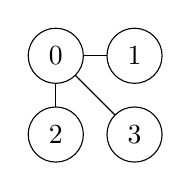
\begin{tikzpicture}
        \draw (0,1) -- (0,0);
        \draw (0,1) -- (1,0);
        \draw (0,1) -- (1,1);
        \foreach \x in {0,1} \foreach \y in {0,1}
            \draw (\x,\y) node[circle,draw,fill=white,inner sep=0,minimum size=0.7cm] {\pgfmathparse{int(2-2*\y+\x)}\pgfmathresult};
        \end{tikzpicture}
    \end{wrapfigure}
    
    Schauen wir uns das Beispiel rechts an.  Hier ist jede Kreuzung eine gute Startposition für den Gendarmen.
    Startet er in Kreuzung 0, kann er im ersten Zug warten; der Räuber muss sich dann zu ihm bewegen.
    Startet er in einer anderen Kreuzung, kann er warten, bis der Räuber auf Position 0 ist, und sich dann dorthin bewegen.
    
    In diesem Beispiel könnten die Funktionen also wie folgt aufgerufen werden:

    \begin{tabular}{|l|c|}
        \hline
            {\bf Funktionsaufruf} & {\bf Liefert} \\
        \hline
            \method{start(4, [[0, 1, 1, 1], [1, 0, 0, 0], [1, 0, 0, 0], [1, 0, 0, 0]])} &
            \constant{3} \\
        \hline
            \method{nextMove(1)} & \constant{3} \\
        \hline
            \method{nextMove(0)} & \constant{0} \\
        \hline
    \end{tabular}

    \Scoring

    \begin{description}
        \item[Teilaufgabe 1 (16 Punkte):] $2 \le N \le 500$. 
        Zwischen je zwei Kruezungen gibt es genau einen Weg.
        \item[Teilaufgabe 2 (14 Punkte):] $2 \le N \le 500$. 
        Die Kreuzungen und Straßen bilden ein Raster.  Das Raster hat mindestens zwei Reihen und Spalten,
        und die Nummerierung der Kreuzungen folgt dem unten abgebildeten Muster.
        \begin{figure}[h!]
           \centering
           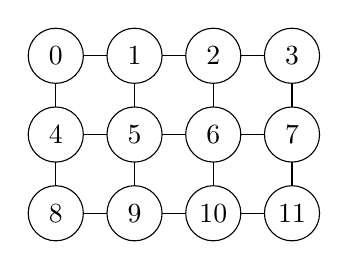
\begin{tikzpicture}
            \draw (0,0) grid (3,2);
            \foreach \x in {0,1,2,3} \foreach \y in {0,1,2}
                \draw (\x,\y) node[circle,draw,fill=white,inner sep=0,minimum size=0.7cm] {\pgfmathparse{int(8-4*\y+\x)}\pgfmathresult};
           \end{tikzpicture}
        \end{figure}
        \item[Teilaufgabe 3 (30 Punkte):] $2 \le N \le 100$.
        \item[Teilaufgabe 4 (40 Punkte):] $2 \le N \le 500$.
    \end{description}
    
    Um volle Punktzahl zu erhalten, muss dein Programm folgende Bedingungen erfüllen
    \begin{enumerate}
    	\item korrekt bestimmen, ob der Gendarm den Räuber fangen kann; und
	\item Züge angeben, mit denen der Gendarm den Räuber fangen kann.
    \end{enumerate}
    
    In Subtasks 3 und 4 erhalten Lösungen, 
    die nur die erste Anforderung erfüllen, 30\% der Punkte.
    
    In Teilaufgabe 1 und 2 muss dein Programm beide Bedingungen erfüllen, um Punkte zu erhalten.
    In Teilaufgabe 3 und 4 genügt die erste Bedingung, um 30\% der Punkte zu bekommen.
    Falls deine Lösung nur auf Teilpunkte abzielt, kann dass Programm also einfach beendet werden indem \method{nextMove} einen ungültigen Wert zurückgibt (z.B. $-1$).

    \Constraints
    
    \begin{description}
        \item[Time Limit:] 1,5 s.
        \item[Memory Limit:] 256 MB.
    \end{description}

    \Experimentation
    Der Beispiel-Grader auf deinem Rechner liest Daten von der Standard-Eingabe.
    Die erste Zeile der Eingabe sollte aus der Anzahl $N$ der Kreuzungen bestehen.
    Die folgenden $N$ Zeilen sollten die Adjazenzmatrix $A$ enthalten.
    Jede dieser Zeilen sollte $N$ Zahlen enthalten jeweils $0$ oder $1$.
    Die Matrix muss symmetrisch sein und die Einträge auf der Hauptdiagonale müssen alle $0$ sein.

    Die nächste Zeile sollte eine Zahl enthalten: $1$, falls die Genarmerie den Räuber fangen kann, andernfalls $0$.
    
    Schlussendlich soll im Fall, dass der Gendarm den Räuber fangen kann, sollten $N$ Zeilen folgen, die die Strategie des Räubers beschreiben. Jede Zeile sollte $N+1$ Zahlen zwischen $0$ und $N-1$ einschließlich enthalten. Der Wert in Zeile $r$ und Spalte $c$ wobei $c<N$ beschreibt durch Angabe einer Kreuzungsnummer, wohin der Räuber in der Situation zieht, in der der Räuber am Zug ist, der Gendarm an Kreuzung $r$ und der Räuber an Kreuzung $c$ steht. Die Werte auf der Hauptdiagonale werden ignoriert, da sie Situationen entsprechen, in denen der Räuber bereits verloren hat. Der Eintrag für $c=N$ in jeder Zeile $r$ gibt an, wo der Räuber in Abhängigkeit von der Startposition $r$ des Gendarms startet.
    
    Eine Beispieleingabe für den Beispiel-Grader mit drei Kreuzungen, die jeweils miteinander verbunden sind:

    \begin{center}
        \begin{tabular}{p{4cm}}
            {\tt
                3 \newline
                0 1 1 \newline
                1 0 1 \newline
                1 1 0 \newline
                1 \newline
                0 2 1 2 \newline
                2 0 0 2 \newline
                1 0 0 1 \newline
            }
        \end{tabular}
    \end{center}

    Die folgende Eingabe passt zum oben angegebenen Beispiel:

    \begin{center}
        \begin{tabular}{p{4cm}}
            {\tt
                4 \newline
                0 1 1 1 \newline
                1 0 0 0 \newline
                1 0 0 0 \newline
                1 0 0 0 \newline
                1 \newline
                0 0 0 0 1 \newline
                2 0 0 0 2 \newline
                3 0 0 0 3 \newline
                1 0 0 0 1 \newline
            }
        \end{tabular}
    \end{center}
\end{document}
